\documentclass[a4paper,oneside,article]{memoir}
\usepackage[UTF8]{inputenc}
\usepackage[Danish]{babel}
\usepackage[T1]{fontenc}

\setsecnumdepth{subsection}
\setcounter{tocdepth}{5}
\setcounter{secnumdepth}{4}

\setsecnumdepth{subsection}
\usepackage{lmodern}
\usepackage{parskip}

%Billeder skal
\usepackage{graphicx}
\graphicspath{ {Afsnit/} }
\usepackage{float}
\usepackage{wrapfig}

% Listings og color bruges til at vise vores VHDL kode med.
\usepackage{listings}
\usepackage{color}

\definecolor{dkgreen}{rgb}{0,0.6,0}
\definecolor{gray}{rgb}{0.5,0.5,0.5}
\definecolor{mauve}{rgb}{0.58,0,0.82}

\lstset{frame=tb,
  language=C++,
  aboveskip=3mm,
  belowskip=3mm,
  showstringspaces=false,
  columns=flexible,
  basicstyle={\small\ttfamily},
  numbers=none,
  numberstyle=\tiny\color{gray},
  keywordstyle=\color{blue},
  commentstyle=\color{dkgreen},
  stringstyle=\color{mauve},
  breaklines=true,
  breakatwhitespace=true,
  tabsize=3
}



\title{Proces Rapport 3. Semesterprojekt - Goofy Candy Gun\\ Gruppe 3}

\author{
  Rieder, Kasper\\
  \texttt{201310514}
  \and
  Jensen, Daniel V.\\
  \texttt{201500152}
  \and
  Nielsen, Mikkel\\
  \texttt{201402530}
  \and
  Kjeldgaard, Pernille L.\\
  \texttt{PK94398}
  \and
  Konstmann, Mia\\
  \texttt{201500157}
  \and
  Kloock, Michael\\
  \texttt{201370537}
  \and
  Rasmussen, Tenna\\
  \texttt{201406382}
}

\pagestyle{headings}

\begin{document}
	
	\frontmatter
	\maketitle

	\clearpage
	\newpage
	
	\tableofcontents
	
	\newpage
	\listoffigures
	\newpage
	
	\mainmatter
	
	\chapter{Forord}
Forord
I denne rapport vil produktet Goofy Candygun 3000 blive beskrevet. Goofy Candygun 3000 er udviklet i forbindelse med semesterprojektet på tredje semester på IHA.

\section{Praktisk information}
Gruppen, der har udviklet Goofy Candygun 3000, består af følgende syv personer: Kasper Rieder, Daniel Vestergaard Jensen, Mikkel Nielsen, Tenna Rasmussen, Michael Kloock, Mia Konstmann og Pernille Kjeldgaard. Gruppens vejleder er Gunvor Kirkelund. Rapporten skal afleveres fredag d. 27. maj 2016 og skal bedømmes ved en mundtlig en eksamen d. 22. juni 2016. Produktet dokumenteres foruden denne rapport med en procesrapport, et dokumentationsdokument, en prototype og diverse bilag. 

\section{Læsevejledning}

	\chapter{Indledning}
Hensigten med dette projekt, er at udvikle spillet "Goofy Candygun 3000". Spillet går ud på at 1-2 spillere dyster om, at ramme et mål med slik, affyret fra en slikkanon, styret af en Wii-Nunchuck controller. For at finde inspiration til projektet, og idéer til implementering, blev der søgt efter lignende projekter på internettet. Det viste sig, at idéen med at skyde med slik, ikke er en original idé, da lignende projekter såsom "The Candy Canon" \cite{Website:CandyCanon} allerede findes. Til forskel fra The Candy Cannon og lignende projekter som affyrer projektiler uden et egentlig formål, vil der i dette projekt blive udviklet en kanon til brug i et spil. Kanonen affyres og styres af spillerne via en controller. Altså skal projektet ende med en kanon som indgår i et to personersspil, f.eks. til brug ved fester og andre sociale begivenheder.
Målet med projektet, er at bygge en funktionelt prototype, samt at dokumentere dette med en projektrapport og dens dertilhørende dokumentation. 
Det følgende afsnit beskriver, hvilke krav der stilles til projektet fra IHA's side.

\section{Krav til produktet}
Projektet tager udgangspunkt i projektoplægget for 3. Semester projektet, præsenteret af \textit{Ingeniørhøjskolen, Aarhus Universitet}. Til dette projekt er der ikke stillet krav til typen af produkt der skal udvikles, dog er der sat krav til hvad produket skal indeholde. Disse krav er som følger:


\begin{itemize}
	\item{Systemet \textit{skal} via sensorer/aktuatorer interagere med omverdenen}
	\item{Systemet \textit{skal} have en brugergrænseflade}
	\item{Systemet \textit{skal} indeholde faglige elementer fra semesterets andre fag}
	\item{Systemet \textit{skal} anvende en indlejret Linux platform og en PSoC platform}
\end{itemize}

\noindent På baggrund af disse krav er der udarbejdet et produkt, der beskrives i afsnit \ref{afsnit:systembeskrivelse}. \newline

\noindent I dette projekt bliver produktet opbygget som en prototype. Grundet dette er der i afsnit \ref{afsnit:analyse} beskrevet nogle grundlæggende hardwarekomponenter til realisering af denne prototype.


\section{Systembeskrivelse}
\label{afsnit:systembeskrivelse}
I dette projekt skal der udvikles en slik kanon, som skal bruges i et nyt spil som kommer til at hedde \textit{Goofy Candygun 3000}. Denne slik kanon skal kunne skyde med slik, eksempelvis M\&M’s eller Skittles. Kanonen der afyrer slikket, skal styres af spillerne via en Wii-Nunchuck controller.  \newline

\noindent Et typisk brugerscenarie er, at spillerne bestemmer antallet af skud for runden. Når dette er gjort, er spillet igang. Herefter går Wii-nunchucken på skift mellem spillerne for hvert skud. Dette fortsættes indtil skuddene er opbrugt. Vinderen er spilleren med flest point. Spillets statistikker vises løbende på brugergrænsefladen. Dette brugerscenarie er illustreret i det rige billede på figur \ref{fig:RigtBillede}.

\begin{figure}[H]
	\centering
	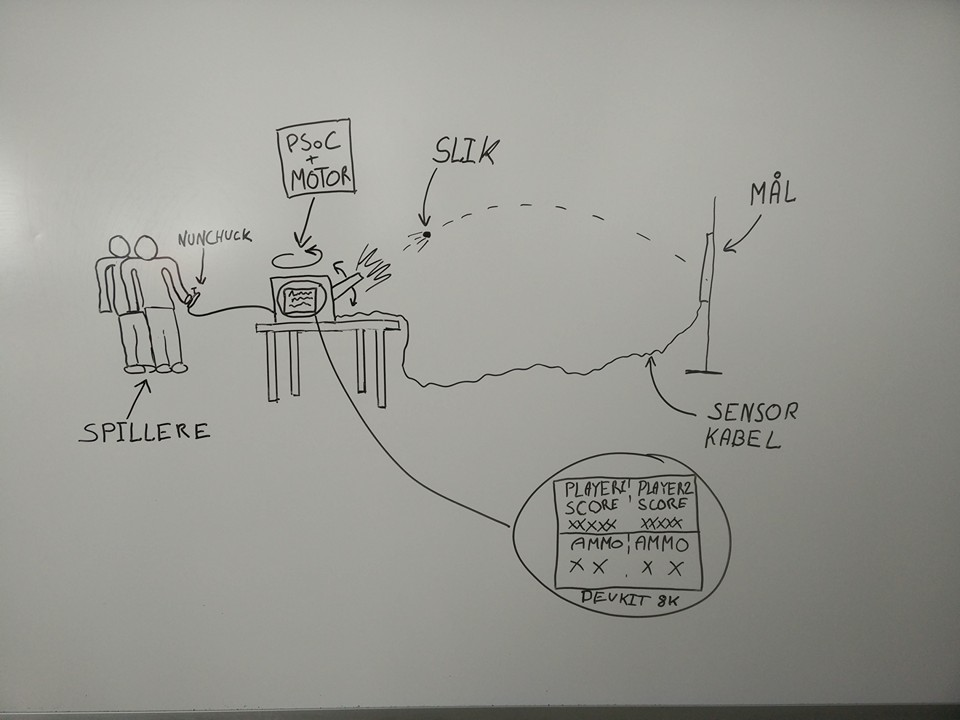
\includegraphics[width=\textwidth]{Projektformulering/images/rigtBillede}
	\caption{Rigt Billede af det endelige produkt}
	\label{fig:RigtBillede}
\end{figure}

Det endelige produkt omfatter:
\begin{itemize}
	\item{En brugergrænseflade, hvor brugeren kan initiere både system test og selve spillet. Derudover kan brugergrænsefladen vise:}
	\subitem{Point}
	\subitem{Kanonens vinkel}
	\subitem{Antal resterende skud}
	\item{Består af 3 motorer, der drejer kanonen om forskellige akser}
	\subitem{Disse skal styres med en Wii-nunchuck controller}
	\subitem{To af motorerne styre kanonen i forskellige retninger og den sidste er til at afyrer kanonen}
	\item{Et mål, der kan registrere spillernes skud}
	\item {Der skal være mulighed for at flere spille kan spille sammen, i stedet for kun 2}
\end{itemize}


%\section{Ansvarsområder}
%I løbet af projektet vil projektgruppen blive opdelt i to hovedgrupper - 'hardware' og 'software'. Softwaregruppen vil desuden stå for grænsefladeprogrammering mellem software og hardware. Disse grupper vil have til ansvar at designe og implementere hhv. hardware og software til projektet. Hardwaregruppen vil bestå af de personer, der læser til elektroingeniør (Mikkel Nielsen og Pernille Kjeldgaard). Softwaregruppen vil bestå af de personer, der læser til IKT-ingeniør (Kasper Rieder, Michael Kloock, Tenna Rasmussen, Mia Konstmann og Daniel Jensen).

	%\chapter{Udviklingsmodel}
I dette afsnit beskrives den udviklingsmodel der anvendes i forbindelse projektets forløb. I dette projekt er der blevet gjort brug af SCRUM som udviklingsmetode.

	\section{Rollebeskrivelser}
	Der er tre hovedroller i scrum; produktejeren, udviklingsholdet og scrum masteren. Disse tre roller udgør scrum teamet. Under dette projekt har gruppevejlederen fungeret som produktejeren, udviklingsholdet har bestået af projekt gruppen og rollen som scrum masteren er varetaget af forskellige medlemmer af gruppen.
	
	\subsection{Produktejer}
	Når der udvikles et produkt er der som regel en produktejer, der har stor interesse i det endelige produkt. Produktejeren definerer rammerne omkring produktet og prioriterer vigtigheden af opgaver på backloggen. \newline
	
	I dette projektforløb er rollen som produktejer en kunstig rolle, i den forstand at gruppen har sat rammerne omkring projektet og prioriterer opgaver under forløbet. Gruppens vejleder har påtaget sig rollen som produktejer, men har meget lidt indflydelse på udkommet af projektet. Til sprintenes afslutnings møder fungerede vejlederen som en konventionel produktejer. Her blev resultaterne af sprintet fremført for produktejeren, som skulle forholde sig kritisk i forhold til resultaterne.
	
	Under et sprintplanlægningsmøde havde produktejeren en reel indfyldelse på prioritering og opgaverne på sprintbackloggen. Inden mødet med produktejeren havde gruppen afholdt et møde og udvalgt de vigtigste opgaver til sprintet. Herefter blev mødet med produktejeren afholdt, som hjalp med prioriteringen af opgaver og gav foreslag til opgaver, der ikke var taget højde for.  
	
	\subsection{Udviklingshold}
	Udviklingsholdet består af en gruppe individer, der arbejder mod et samlet mål; et færdigt delprodukt for hvert sprint. Udviklingsholdet er selvorganiserende, dermed udpeges der ikke nogen holdleder. \newline
	
	I dette projekt bestod udviklingsholdet af gruppemedlemmerne, der hver især har forskellige egenskaber der giver værdi til holdet. Det er udenfor normerne at scrum masteren er en del af udviklingsholdet. Dette er dog tilfældet under dette projektforløb, da det ville hindre projektet at udelade en person fra udviklingsholdet på grund af sin rolle som scrum master. \par
	Under førløbet har udviklingsholdet været mere eller mindre selv organiseret med lille indflydelse af højere instanser. Der er dog nogle deadlines og krav, der skulle overholdes fra IHA's side.
	
	
	\subsection{Scrum master}
	En af hovedrollerne i scrum er scrum masteren. Scrum masterens vigtigste rolle er at sikre at processen i projektforløbet er bevaret. Med dette menes at scrum masteren skal sørge for at udviklingsholdet overholder reglerne for scrum ved at coache dem i at anvende scrum. Derudover skal scrum masteren fungere som bindeled mellem produktejeren og udviklingsholdet. Der er mange andre vigtige opgaver som scrum masteren typisk skal varetage sig, så som ordstyrer til daglige morgenmøder, hjælpe holdet med at afgøre hvad der skal udføres i et sprint og holde et alment overblik over gruppens fremskridt. Da scrum anvendes til et semester projekt og ikke et fuldtidprojekt, er der nogle dele af scrum master rollen vi har taget til os, nogle som vi anvender på vores egen måde og nogle som vi ser bort fra. \newline
	
	Under dette projekt overtog et nyt gruppemedlem rollen som scrum master for hvert sprint. Som scrum master havde man to ansvarsområder; holde overblik over logbøgerne og fungere som bindeled mellem produktejeren og udviklingsholdet. \newline
	
	Under projektforløbet blev der ikke afholdt daglige morgenmøder hvor scrum masteren kunne skabe et overblik over gruppen. Dette er blevet erstattet med logbøger, der blev udfyldt hver morgen inden dagens arbejde påbegyndes. Da der ikke arbejdes på projektet så koncentreret som scrum er bygget til, var daglige morgenmøde valgt fra grundet forskellige mødetider i gruppen. \par
	I stedet for at fungere som ordstyrer til morgenmøder, skulle scrum masteren læse hvert gruppemedlems logbog igennem. I disse logbøger blev der besvaret tre spørgsmål og noteret eventuelle bemærkninger. De tre spørgsmål, er de samme tre spørgsmål, man ville blive spurgt hvis der var afholdt morgenmøderne:
	
	\begin{itemize}
		\item Hvad lavede du i går?
		\item Hvad skal du lave i dag?
		\item Skal der bruges hjælp?
	\end{itemize} 
	
	Hvis der var opstået problemer for en af gruppens medlemmer var det scrum masterens ansvar at reagere på det. I og med at scrum masteren ikke har nogen reel ansvar for gruppen eller på produktet, har scrum masteren ikke noget ansvar til at løse problemerne. Derimod er scrum masteren med til at afhjælpe problemet ved at gøre resten af gruppen opmærksom på de nyopstandne problemer. 
	
	Som bindeled skulle scrum masteren kommunikere med produktejeren, som i dette tilfælde var gruppens vejleder. Til sprintplanlægningsmøder skulle gruppen bestemme hvad der skulle foretage i det næste sprint. Ved rigtig anvendelse af scrum ville produktejeren være til stede til disse møder for at få afstemt forventninger omkring det næste sprint. Derefter ville scrum masteren, med produktejerens ønsker i tankerne, sætte opgaver på sprintbackloggen sammen med udviklingsholdet. Da dette ville være en tidskrævende process, blev det bestemt at vejlederens tilstedeværelse ikke var nødvendig til denne process og blev først konsulteret efter backloggen var blevet udfyldt med opgaver. Til møderne fungerede scrum masteren som ordstyrer og oprettede opgaver på Pivitol Tracker efter gruppens ønsker. \par 
	Under forløbet er gruppens dokumenter til dokumentationsrapporten blevet reviewet af en anden gruppe. Her skulle scrum masteren samle dokumenterne, der skulle reviewes, og lave mødeindkaldelser til reviewmøderne.
	
	
	
	\section{Udfordringer ved anvendelse af scrum}
	I forbindelse med at det er første gang, der anvendes scrum til et semester projekt, er dele af scrum som vi har haft udfordringer med at få inddraget i udviklingsprocessen, hvilket har hindret processen. \newline
	
	\subsection{Kommunikation}
	En vigtig del af scrum er kommunikation. Da gruppen bestod af medlemmer fra forskellige studieretninger, var det ikke muligt at afholde daglige morgen møder, og dette var en stor hindring for kommunikationen. Gruppensmedlemmer havde ikke overblik over hvad der foregik end det man selv var i gang med. Som kommunikationsværktøj blev der oprettet en Facebook gruppe. Her kunne gruppens medlemmer aftale arbejdsdage og informere hinanden om vigtige ting. Dette værktøj blev ikke anvendt så godt som det kunne have gjort, dermed skete der en del miskommunikation omkring arbejdsdage og hvornår man skulle mødes. \par
	Det er ikke muligt for grupper på tredje semester at få et grupperum. Dette ville have gjort en del for kommunikation at man havde et fælles møderum, hvor der kunne arbejdes og hvor scrumboardet kunne placeres. Da dette ikke var en mulighed blev scrumværktøjet Pivitol Tracker anvendt. Der var uklarhed om hvordan dette værktøj skulle anvendes og det tog et par sprint før dette blev afklaret. Her ville det have været en fordel at have et scrumboard med sticky notes, som man arbejder normalt i scrum. 
	
	\subsection{Sprintbackloggen}
	Anvendelsen af Pivitol Tracker's backlog gik galt fra starten, da der ikke blev lavet en veldefineret liste. For hvert sprint blev der lavet nye opgaver alt efter gruppens ønsker til det kommende sprint. Det at der ikke en veldefineret backlog betød at der ikke kunne udvælges opgaver derfra, da disse opgaver ført blev definieret da vi kom i tanke om dem. \par
	Under sprintplanlægningsmøderne manglede der struktur og der blev ikke aflagt nok tid til at afholde disse møde. Dette betød at opgaver ikke var veldefineret og disse blev ændret i løbet af sprintet, som er noget der ikke må ske når der køres et sprint. Udover at opgaverne ikke var veldefineret, var der opgaver der ikke var taget højde for. Dermed blev der arbejdet på opgaver, der ikke var på sprintbackloggen og tog tid væk fra de tidsestimerede opgaver. Dette førte til at alle opgaver op sprintbackloggen aldrig blev fuldtført og tidsplanen blev ved med at skride.  

	\chapter{Udviklingsmodel - Scrum}
Under dette projektforløb er scrum udviklingsmodellen brugt til processtyring. Denne udviklingsmodel er en iterativ metode der bruges til styring, organisering og planlægning af produkt udviklingen.

%I dette afsnit beskrives den udviklingsmodel der anvendes i forbindelse projektets forløb. I dette projekt er der blevet gjort brug af scrum som udviklingsmetode.

\section{Rollebeskrivelser}
Der er tre hovedroller i scrum \cite{scrumGuides}; produktejeren, udviklingsholdet og scrum masteren. Disse tre roller udgør scrumteamet. Under dette projekt har gruppevejlederen fungeret som produktejeren, udviklingsholdet har bestået af projektgruppen og rollen som scrum master er skiftevis varetaget af forskellige medlemmer af gruppen.

\subsection{Produktejer}
Når der udvikles et produkt er der som regel en produktejer, der har stor interesse i det endelige produkt. Produktejeren definerer rammerne omkring produktet og prioriterer vigtigheden af opgaver på backloggen. \cite{scrumGuides} \newline

\noindent I dette projektforløb er rollen som produktejer en kunstig rolle, i den forstand at gruppen har sat rammerne omkring projektet og prioriterer opgaver under forløbet. Gruppens vejleder har påtaget sig rollen som produktejer, men har meget lidt indflydelse på udkommet af projektet. Til sprintenes afslutningsmøder fungerede vejlederen som en konventionel produktejer. Her blev resultaterne af sprintet fremført for produktejeren, som skulle forholde sig kritisk i forhold til resultaterne.\newline 

\noindent Under et sprintplanlægningsmøde havde produktejeren en reel indfyldelse på prioritering af opgaver, og opgaverne på sprintbackloggen. Inden mødet med produktejeren havde gruppen afholdt et møde og udvalgt de vigtigste opgaver til sprintet. Herefter blev mødet med produktejeren afholdt, som hjalp med prioriteringen af opgaverne og gav forslag til opgaver, der ikke var taget højde for.  \newline 

\noindent Vejlederens forudsætning for at prioritere de opgaver, der skulle løses i det kommende sprint var at prioritere de læringsmål, der er opstillet i kursusbeskrivelsen \cite{laeringsmaal}. Det var altså vejlederens opgave at vejlede gruppen, så der ved afslutningen af projektet ville være opfyldt så mange læringsmål som muligt. Læringsmålene skulle afspejles i prioriteringen af opgaver i sprintbackloggen. 

\subsection{Udviklingshold}
Udviklingsholdet består af en gruppe individer, der arbejder mod et samlet mål - et færdigt delprodukt for hvert sprint. Udviklingsholdet er selvorganiserende, og dermed udpeges der ikke nogen holdleder. \cite{scrumGuides} \newline

\noindent I dette projekt bestod udviklingsholdet af projektets gruppemedlemmer, der hver især har forskellige egenskaber, der giver værdi til holdet. Det er udenfor normerne, at scrum masteren er en del af udviklingsholdet. Dette er dog tilfældet under dette projektforløb, da det ville hindre projektet, at udelade en person fra udviklingsholdet på grund af sin rolle som scrum master. \newline

\noindent Under førløbet har udviklingsholdet været mere eller mindre selvorganiseret. Der har dog været nogle deadlines og krav, der skulle overholdes fra IHA's side.

\subsection{Scrum master}
En af hovedrollerne i scrum er scrum masteren. Scrum masterens vigtigste rolle er at sikre, at processen i projektforløbet er bevaret \cite{scrumGuides}. Med dette menes, at scrum masteren skal sørge for at udviklingsholdet overholder reglerne for scrum ved at coache dem i at anvende scrum. Derudover skal scrum masteren fungere som bindeled mellem produktejeren og udviklingsholdet. Scrum masterens fornemmeste opgave er altså at facilitere scrumprocessen for gruppens medlemmer. \newline

\noindent I dette projekt har der været en række administrative opgaver, som vi har valgt at tildele scrum masteren. Derfor har scrum masteren i vores projekt også fungeret som en sekretær for gruppen. Dette har blandt andet indebåret at indkalde til vejledermøder, fungere som ordstyrer til disse møder, holde overblik over gruppens arbejde og fremskridt og holde overblik over de daglige opdateringer i logbøgerne. \newline

\noindent I dette projekt har det også været scrum masterens opgave at være ordstyrer for de daglige stå-op-møder i den uge, der blev gjort brug af disse. Det har også været scrum masterens opgave at sørge for at skaffe hjælp, når der opstod problemer med en opgave. Det er ikke scrum masterens opgave at løse problemerne selv, men derimod at synliggøre problemet for teamet. \newline

\noindent Som bindeled skulle scrum masteren kommunikere med produktejeren, som i dette tilfælde var gruppens vejleder. Til sprintplanlægningsmøder skulle gruppen bestemme, hvad der skulle foretages i det næste sprint. Ved rigtig anvendelse af scrum ville produktejeren være til stede til disse møder for at få afstemt forventninger omkring det næste sprint \cite{scrumProductOwner}. Derefter ville scrum masteren, med produktejerens ønsker i tankerne, sætte opgaver på sprintbackloggen sammen med udviklingsholdet. Da dette ville være en tidskrævende process, blev det bestemt, at vejlederens tilstedeværelse ikke var nødvendig til denne proces og blev først konsulteret efter backloggen var blevet udfyldt med opgaver. Til disse møder fungerede scrum masteren som ordstyrer og oprettede opgaver på Pivotal Tracker (se afsnit \ref{section:pivotalTracker}) efter gruppens ønsker. 

\newpage
\chapter{Projektgennemførsel}
I følgende afsnit beskrives essentielle redskaber der er blevet gjort brug af til gennemførelse af projektet. 

\section{Samarbejdsaftale}
For at få et godt projekt, og en god oplevelse i projektgruppen, blev der udarbejdet en samarbejdskontrakt (Bilag/Procesrapport/Samarbejdsaftale.pdf). Denne indeholder aftaler i forhold til forventning af mødedeltagelse, gruppeledelse, og ambitioner for selve projektet. Samarbejdsaftalen blev udarbejdet før at det blev besluttet at bruge scrum, og er ikke blevet revideret siden.

\section{Arbejdsfordeling}
Som udgangspunkt blev gruppen opdelt i to hovedgrupper: en softwaregruppe bestående af Mia, Michael, Kasper, Tenna og Daniel; og en hardwaregruppe bestående af Mikkel og Pernille. Denne inddeling skete på baggrund af studieretning, og dermed som resultat af interesser og kompetencer. I tilfælde hvor der opstod faglige problemer, var opdelingen ikke mere fastsat end at gruppens medlemmer kunne hjælpe hinanden på tværs af hovedgrupperne.

\section{Projektledelse}
Scrum er en udviklingsmodel, der ikke understøtter en projektleder i en traditionel forstand \cite{scrumGuides}. Der har for hvert sprint været en ny scrum master der skulle holde overblik over scrumprocessen. Under dette projektforløb har der været brug for en til at styre opgaver som sekretær og mødeleder. Derfor forekom det gruppen naturligt, at scrum masteren overtog dette ansvar udover sin rolle som scrum master.

\section{Møder}
Gennem hele projektforløbet har der været afholdt et ugentligt vejledermøde. Dette møde har undertiden været brugt til at afholde review- og retrospectivemøder i forbindelse med scrum. Til hvert vejledermøde, blev der udarbejdet en dagsorden, der kunne bruges som udgangspunkt for referatet af mødet. (Bilag/Procesrapport/Møder/) Ved hvert møde blev det aftalt, hvornår det næste vejledermøde skulle afholdes.\newline

\noindent En central del af scrum, er de daglige stå-op-møder \cite{scrumGuides}. Disse har været en udfordring for os at holde, idét at vi har haft forskellige mødetider i løbet af dagen. For at løse dette problem har vi prøvet flere alternativer. Først prøvede vi at bruge logbøger, hvor scrum masteren havde til opgave at kigge logbøgerne igennem for at finde eventuelle problemer. I logbøgerne skulle følgende spørgsmål besvares:

\begin{itemize}
	\item Hvad lavede du i går?
	\item Hvad skal du lave i dag?
	\item Skal der bruges hjælp?
\end{itemize} 

Gruppen erfarede, at logbøgerne ikke var optimale for udførslen af scrum og blev derfor enige om at prøve at afholde fysiske stå op møder hver dag i en uge. Det var udfordrende at få disse til at hænge sammen med alle gruppemedlemmers skemaer, så derfor blev der oprettet en gruppesamtal på facebook. Her skulle alle gruppens medlemmer hver morgen skrive det samme, som skulle skrives logbøgerne. Det blev erfaret, at måden med at afholde stå op møder over Facebook fungerede bedst, og denne metode blev derfor anvendt i resten af projektforløbet. Denne måde at afholde møderne på gav et hurtigt overblik over, hvad alle gruppemedlemmer havde lavet, hvilke planer de havde for dagen. 

\section{Projektadministration}
Under dette projekt er der anvendt nogle værktøjer til at administrere projektet. Værktøjerne er alle internetbaseret, da disse skulle være lettilgængelige for alle gruppemedlemmer, og kunne anvendes på trods af manglende fast grupperum.

\subsection{GitHub}
Til projektet var det vigtigt at have samlet alle projektets filer og dokumenter, således at alle gruppemedlemmer kunne tilgå, og redigere i filerne. Det var også af stor betydning, at der blev holdt en automatisk versionshistorik for alle filer, så alle ændringer blev dokumenterede. Til dette brugte vi versionsstyrings softwaret \textit{Git}, via \textit{GitHub} \cite{git} \cite{gitRepo}. GitHub er en webbaseret løsning, der stiller en gratis Gitserver til rådighed, samt en brugergrænseflade for at kunne tilgå de uploadede filer. \newline

\noindent På figur \ref{ref:GitHubHistorik} ses et udsnit af en versionshistorik for et af projektets filer. Her kan det ses, at ændringer i filen bliver associeret med et gruppemedlem, en kort beskrivelse af ændringen, samt datoen for ændringen.

\begin{figure}[H]
	\centering
	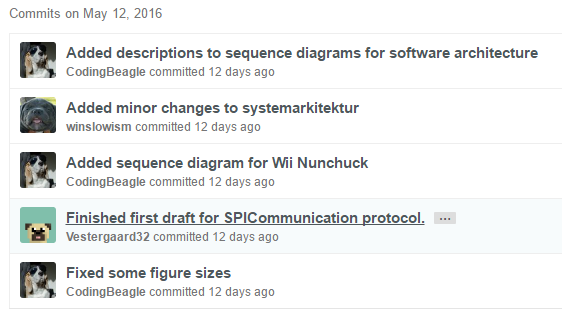
\includegraphics[width=\textwidth]{Projektgennemfoerelse/images/GitHubHistorik}
	\caption{Versionshistorik for et af projektets filer}
	\label{ref:GitHubHistorik}
\end{figure}

\noindent Måden hvorpå gruppen har brugt Git, er at hvert medlem har synkroniseret lokale ændringer løbende til den centrale server. Ved at gøre dette er den nyeste version af projektet altid tilgængeligt for alle andre. \newline

\noindent Git har været en stor hjælp. Det fungerer som en god sikkerhedsmekanisme, da der altid findes en online backup af projektet, samt ældre revisioner. Versionshistorikken er med til at danne et godt overblik over, hvad alle medlemmer arbejder på og retter i. Ved nogle punkter i projektforløbet blev versionshistorikken også brugt til at gendanne tidligere versioner af filer, hvis der ved uheld var introduceret fejl i for eksempel softwarekomponenter. \newline

\noindent En af de negative sider ved at bruge Git, var at gruppen ikke havde erfaring med værktøjet. Derfor skulle der bruges meget tid på at lære at bruge det effektivt. Efterhånden som der blev opnået større erfaring med brugen af Git, endte det med at være et meget værdifuldt værktøj for projektet.  

\subsection{Pivotal Tracker}
\label{section:pivotalTracker}
For at have et scrum board på nettet, som alle kunne tilgå blev Pivotal Tracker \cite{pivotalTracker} anvendt. Pivotal Tracker er et professionelt scrumværktøj, der indeholder mange funktioner. Det er blandt andet scrumboardet, grafer over for eksempel burndowncharts og statistikker. Programmet blev valgt ud fra en anbefaling fra vores vejleder.

\begin{figure}[H]
	\centering
	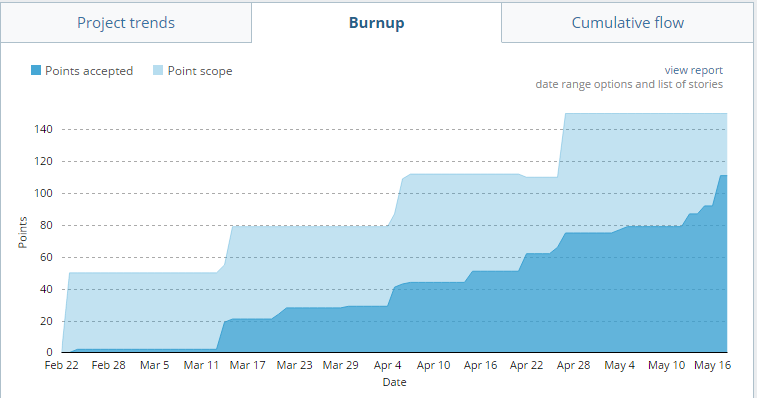
\includegraphics[width=\textwidth]{Projektgennemfoerelse/images/burnupchart}
	\caption{Autogenereret burnup chart fra Pivotal Tracker}
	\label{fig:burnup}
\end{figure}

\noindent På figur \ref{fig:burnup} ses et burnup chart fra Pivotal Tracker, taget for hele gruppens projektforløb. Denne burnup chart viser hvor mange point der er færdiggjort igennem forløbet.

\subsection{Facebook}
Til kommunikation mellem gruppensmedlemmer blev der oprettet en Facebook \cite{facebook} gruppe. Denne gruppe blev brugt til lave aftaler, fildeling og almen kommunikation. Dette værktøj var en essentiel del af gruppekommunikationen. Alle gruppemedlemmerne havde en forhåndsviden om facebook, og der skulle derfor ikke bruges tid på at lære et nyt værktøj. \newline

\noindent Da der skulle aftales arbejdsdage for påsken blev der oprettet en afstemmning. Med denne afstemmning fik hvert medlem tilkendegivet hvilke dage de havde til rådighed. Resultatet af afstemmningen var de to dage der havde størst opbakning. Dette ses i figur \ref{ref:fbpoll}, som er et udsnit af afstemningen.
\begin{figure}[H]
	\centering
	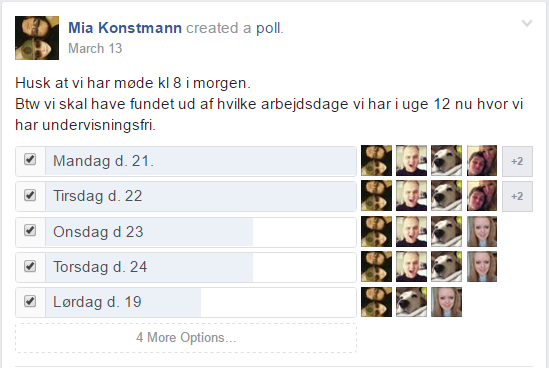
\includegraphics[scale=0.6]{Projektgennemfoerelse/images/fbpoll}
	\caption{Afstemning omkring arbejdsdage}
	\label{ref:fbpoll}
\end{figure}

\noindent Facebook gruppen fungerede som en opslagstavle, hvor der kunne dele informationer og meddele hinanden omkring hvordan dokumentation skulle håndteres. Under dette projekt er der blevet brugt LateX til dokumentation. Dermed skulle der lave aftaler omkring hvordan referencer skulle håndteres, når det afsnit man refererede til endnu ikke var skrevet. På figur \ref{ref:fblatex} ses, at løsningen til dette problem beskrives med en vejledning omkring hvordan referencer skal håndteres.

\begin{figure}[H]
	\centering
	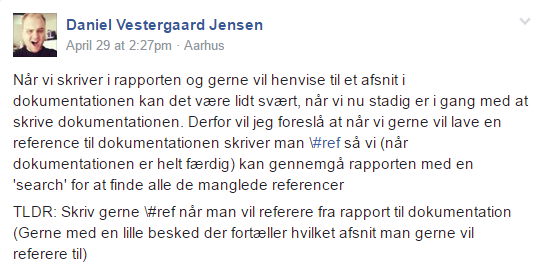
\includegraphics[scale=0.6]{Projektgennemfoerelse/images/fblatex}
	\caption{Opslag omkring referencer}
	\label{ref:fblatex}
\end{figure}

\noindent Til at erstatte stå op møderne og logbøger er der blevet oprettet en gruppesamtale. I denne chat informerede man hinanden omkring det der var foretaget dagen før og det der skulle foretages på dagen. Et udsnit af denne samtale ses på figur \ref{ref:fbchat}. Denne form for kommunikation fungerede bedre end de andre forsøg der var blevet gjort på at holde daglige stå op møder. 

\begin{figure}[H]
	\centering
	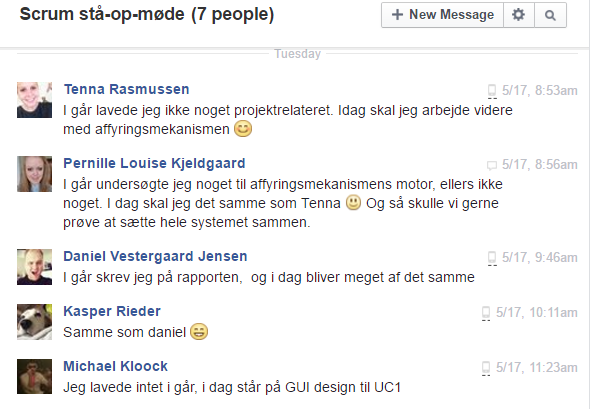
\includegraphics[scale=0.6]{Projektgennemfoerelse/images/fbstandup}
	\caption{Udsnit af gruppesamtalen}
	\label{ref:fbchat}
\end{figure}
\newpage
\noindent Til dette projekt har Facebook været et vigtigt kommunikationsværktøj. Det blev muligt for gruppens medlemmer at kommunikere med hinanden på trods af varierende undervisningstimer og personlige skemaer. Ved at bruge Facebook påmindede man hinanden om at opretholde kommunikationen når man fik en notifikation på sin startside.

\chapter{Scrumkursus ved Systematic}
Som en del af projektet deltog gruppens medlemmer i et scrumkursus som udbydes af Systematic. Som udgangspunkt havde gruppen arbejdet med scrum i to måneder inden kursets start, dermed var der en forforståelse af hvordan scrum skulle anvendes i forbindelse med projektarbejdet. I de følgende afsnit vil de erfaringer som gruppen har gjort sig under kurset blive opsummeret.

\section{Scrum Spillet}
En af øvelserne til kurset var scrum spillet. Her blev gruppen præsenteret med en backlog af små, veldefinerede opgaver. Hver af disse opgaver havde en pointværdi. Når en opgave var fuldført og godkendt af produktejeren, kunne gruppen lægge denne pointværdi til den totale pointsum. Der blev udført tre sprint hver på 15 minutter. Før hvert sprint var der et sprintplanlægningsmøde på 10 minutter og efter hvert sprint var der aflagt fem minutter til retrospective. \newline

\noindent Under sprint planlægningsmøderne valgte gruppen de opgaver, som skulle laves i sprintet. Disse kunne enten udføres individuelt eller i grupper, og hvert gruppemedlem meldte sig selv ind på de opgaver de følte de kunne udføre. Dette betød at hvert medlem havde ansvar for sine egne opgaver, og dermed var der en forpligtelse til at udføre opgaven før sprintets afslutning. \newline

\noindent Under sprintene var der meget samarbejde omkring arbejdsopgaverne. Når et gruppemedlem konstaterede at der ikke var nok tid til at fuldføre en opgave, blev der hurtigt set på hvilke medlemmer der kunne assistere. Her var gruppen god til at holde overblik og være selvorganiserende. I og med opgaverne var veldefinerede, skete der sjældent misforståelser omkring opgavens natur, hvilket betød at arbejdet kunne startes hurtigt. Når der var tvivl omkring opgaverne kunne man konsultere en produktejer som opklarede tvivlen med en klar melding, som gruppen kunne forholde sig til og rette sig efter.  \newline

\noindent Til retrospective fik gruppen talt om hvad der fungerede og hvad der ikke fungerede for sprintet. Under første sprint var der ingen struktur omkring hvordan backloggen var sorteret, og hvor sprintopgaverne var placeret, hvilket skabte forvirring når der var pres på under selve sprintet. Herefter blev der opsat en struktur i form af lommer der var katagoriseret i \textit{Udførte opgaver} og \textit{Backlog}. I \textit{Udførte opgaver} lommen lå godkendte opgaver og i \textit{Backlog} lommen lå de opgaver der endnu ikke var påbegyndt. Disse opgaver var sorteret, så hurtige og lette opgaver lå øverst og kunne tages hvis der ikke var flere opgaver på sprintbackloggen. De sprintopgaver man havde ansvar på fik man i hånden, så man kunne give den til produktejeren når der skulle godkendes en opgave. \newline
Denne øvelse gav os erfaring med, hvor vigtigt det er at have et organiseret arbejdsrum, og veldefinerede opgaver i forbindelse med scrum og sprints.

\section{Perspektivering}
Under dette kursus har gruppen fået en praktisk forståelse omkring brugen af scrum. Vi oplevede at kommunikationen mellem gruppens medlemmer forbedres, når vi er fysisk sammen og har en fysisk og veldefineret sprintbacklog, som vi kan forholde os til. Det ville derfor gavne gruppen at have et grupperum hvor et fysisk scrumboard kunne sættes op. Dermed får vi muligheden for at visualisere de opgaver, der skal udføres i sprintet. \newline

\noindent I modsætning til projektarbejdet var der veldefinerede og simple opgaver for hvert sprint. I projektarbejdet har vi haft problemer med at formulere letforståelige opgaver, hvilket kun skaber forvirring når sprintbackloggen er fastsat, og arbejdet er i gang.\newline

\chapter{Udviklingsforløb}
I bilag (Bilag/Procesrapport/SprintBeskrivelser) ses en detaljeret beskrivelse af hvert sprintforløb, samt erfaringerne gjort under sprintet.

\chapter{Udfordringer ved anvendelse af scrum}
I forbindelse med at det er første gang, vi anvender scrum til et semester projekt, er der dele af scrum som vi har haft udfordringer med at få inddraget i udviklingsprocessen.

\section{Kommunikation}
En vigtig del af scrum er kommunikation. Da gruppen bestod af medlemmer fra forskellige studieretninger, var det ikke muligt at holde daglige stå op møder, hvilket gjorde det uoverskueligt at holde styr på, hvad de andre på teamet lavede. Som kommunikationsværktøj blev der oprettet en Facebook gruppe. Her kunne gruppens medlemmer aftale arbejdsdage og informere hinanden om vigtige hændelser. Dette værktøj blev ikke anvendt så godt som det kunne have været, dermed skete der en del miskommunikation omkring arbejdsdage og mødetider. \newline

\section{Organisering}
Det er ikke muligt for grupper på tredje semester at få et grupperum til semesterprojekt arbejde. Det ville have gjort en del for kommunikationen at have et fællesrum, hvor der kunne arbejdes og hvor scrumboardet kunne placeres. Da dette ikke var en mulighed blev scrumværktøjet Pivotal Tracker anvendt. Der var uklarhed om hvordan dette værktøj skulle anvendes og det tog et par sprint før dette blev afklaret. Her ville det have været en fordel at have et scrumboard med sticky notes, eller eventuelt at gøre brug af et mindre kompliceret værktøj til at holde et online scrum-board. Dette kunne for eksempel være Trello \cite{trello} eller lignende. 

\section{Sprintbackloggen}
Ved anvendelse af Pivotal Tracker's backlog blev der fra start opstillet en række af opgaver. I arbejdet med udviklingen af projektet, blev yderligere tilføjelser dog nødvendige. Her har scrum som agil udviklingsmodel sin fordel, idet, det er muligt at tilføje og ændre i funktionaliteterne for projektet undervejs. 
Grundet manglende erfaring med tidsestimering, har de fleste af sprintbackloggens opgaver været fejlestimerede. Det var en tendens til at udførelsestiden for en opgave blev groft undervurderet. Her kunne det muligvis have været en fordel at have prioriteret mere tid til sprintplanlægninsmøderne, for at få diskuteret opgaverne grundigt igennem. 


\chapter{Perspektivering}
Processtyringen af dette projekt har været præget af en usikkerhed, idét gruppen ikke havde en tidligere erfaring med brugen af scrum. Dette afspejles i de udfordringer gruppen har stødt på under projektforløbet, for eksempel manglende kommunikation, forhastede planlægningsmøder og fejl i tidsestimeringer. Dette har dog ikke forhindret gruppen i at afprøve nye metoder for at afhjælpe disse problemer. \newline

\noindent For at forbedre kommunikationen mellem gruppens medlemmer blev der forsøgt med forskellige metoder såsom logbøgerne og morgenmøderne. Vi oplevede dog at dette først blev forbedret, da Facebook samtalen blev indført. Det gjorde at alle fik en indsigt i hvad andre gruppemedlemmer skulle lave på dagen, og hvad der var blevet lavet dagen forinden. \newline

\noindent Der findes utallige metoder til tidsestimering, såsom estimering med t-shirt størrelser. Under dette projekt blev denne metode anvendt, da denne var et nemt udgangspunkt at starte fra. Det viste sig dog at estimeringerne var fejlvurderet da man ikke havde indsigt i hvor langt tid opgaver tager. T-shirt metoden var en god måde at gør det på, når man ikke har tidsestimeret før. Vi oplevede dog, at jo mere det bruges, jo lettere bliver det at lave nøjagtige tidsestimeringer. Et alternativ til dette er planning poker \cite{planningpoker}, som giver mulighed for flere tidsværdier til hver opgave. Dette kræver dog at man har bedre forståelse for hvor langt tid opgaverne tager og involverer flere diskussioner, når tidsværdierne er spredt over et større interval. 
	\chapter{Konklusion}
Der blev i dette projekt brugt scrum som en udviklingsmodel, da denne model kan håndtere ændringer i krav til produktet eller design under projektforløbet. Derved var det muligt at arbejde iterativt, da man kunne tage hensyn for de nye ændringer i det nye sprint. \newline
\noindent Under dette projektforløb har gruppen fået indsigt i den praktiske anvendelse af scrum.

 For hver sprintopstart blev der bestemt opgaver til udførelse samt tidsestimeret disse opgaver. Det med at der skulle laves sprint, ca 3 uger, gjord at man fik et del mål, man hele skulle nå, så man så småt kunne se at projekt skred frem ad, som havde en positiv effekt på os. I stedet for at det var et stort mål til sidst på semestret, var det godt med små del mål. \\Der skulle i scrum laves stå op møder hver dag, der blev fundet af for gruppen at det funger bedst med facebook chat, hvor man skrev hvad man skulle lave og hvad man har lavet. Så det gav os et større overblik over hvad der sket ved de andre. Så det var noget alle var gælder for det, som vi nok skulle have gjord fra starten af, for at opretholde  en god kommunikation imellem hinanden. igennem projektet har vi fundet en større viden om hvordan scrum funger og hvilke ting som man kan bruge i de projeket her på studiet. 
\\Så alt i alt har scrum nogle gode redskab, som man med sikkerhed vil tage med videre i sit undervisnings forløb her på Århus ingeniørhøjskole 
 



 




	\bibliographystyle{plain}
\bibliography{references}

\end{document}